\noindent
\begin{tabular}{|>{\colleft}p{3cm}|>{\colleft}p{8.5cm}|} \hline
{\bf Communication model} 	& {\bf Information Exchange Specification Worksheet CM-2} \\ \hline \hline
\sc Transaction 			& \emph{Transaction 1: Report complaint}  \\ \hline
\sc Agents involved 		& 1. {\bf Sender}(Hobbyist): Initiate repair  \newline
					  2. {\bf Receiver}(Car repair assistant): Initiate repair \newline
					  3. {\bf Sender}(Car repair assistant): List of components  \newline
					  4. {\bf Receiver}(Hobbyist): List of components \newline
					  5. {\bf Sender}(Hobbyist): Component  \newline
					  6. {\bf Receiver}(Car repair assistant): Component \newline
					  7. {\bf Sender}(Car repair assistant): List of malfunctions  \newline
					  8. {\bf Receiver}(Hobbyist): List of malfunctions \newline
					  9. {\bf Sender}(Hobbyist): Malfunction  \newline
					  10. {\bf Receiver}(Car repair assistant): Malfunction \\ \hline
\multicolumn{2}{|l|}{\textsc{Information items}} \\ \hline
   					%List all information items that are to be transmitted in this
   					%transaction. This includes the (`core') information object the
   					%transfer of which is the purpose of the transaction. However, it may contain
   					%other, supporting, information items, that, for example, provide help
   					%or explanation. For each information item, describe the following:
   
INITIATE REPAIR			&  1. {\bf Role}: A core information object. \newline
					% whether it is a {\em core} object, or a {\em support} item.
					   2. {\bf Form}: A boolean indicating the start of a repair process \newline
					% the syntactic form in which it transmitted to another agent , e.g., data string, canned text, a certain type of diagram, 2D or 3D plot.
					   3. {\bf Medium}: By starting the program using an icon or command\\
					% the medium through which it is handled in the agent-agent interaction, e.g., a pop-up window, navigation and selection within a menu, command-line interface, human intervention.
LIST OF COMPONENTS		&  1. {\bf Role}: A support information object. \newline
					   2. {\bf Form}: A list of strings \newline
					   3. {\bf Medium}: As menu items\\
COMPONENT				&  1. {\bf Role}: A core information object. \newline
					   2. {\bf Form}: An identifier \newline
					   3. {\bf Medium}: As a selection within a menu\\
LIST OF MALFUNCTIONS		&  1. {\bf Role}: A support information object. \newline
					   2. {\bf Form}: A list of strings \newline
					   3. {\bf Medium}: As menu items\\
MALFUCNTION				&  1. {\bf Role}: A core information object. \newline
					   2. {\bf Form}: An identifier \newline
					   3. {\bf Medium}: As a selection within a menu\\ \hline
\multicolumn{2}{|l|}{\textsc{Message specifications}}\\ \hline
					% Describe all messages that make up the transaction. For each individual message describe:
INITIATION-MESSAGE		& {\bf Communication type}: ORDER\newline
					% the communication type of the message describing its intention (``illocutionary force,'' in speech-act terminology). 
					  {\bf Content}: Initiate repair\newline
					% the statement or proposition contained in the message.
					%&  3. {\bf Reference}: \\ \hline
					%in certain cases, it may be useful to add a reference to, for example, what domain knowledge model or agent capability is required to be able to send or process the message.
					  {\bf From}: Hobbyist\newline
					  {\bf To}: Car repair assistant\\
COMPONENT-LIST-MESSAGE		& {\bf Communication type}: ASK\newline
					  {\bf Content}: List of components and the request to chose one\newline
					%&  3. {\bf Reference}: \newline
					  {\bf From}: Car repair assistant\newline
					  {\bf To}: Hobbyist\\
COMPONENT-MESSAGE			& {\bf Communication type}: REPLY\newline
					  {\bf Content}: Component\newline
					%&  3. {\bf Reference}: \\ \hline
					  {\bf From}: Hobbyist\newline
					  {\bf To}: Car repair assistant\\
MALFUNCTION-LIST-MESSAGE	& {\bf Communication type}: ASK\newline
					  {\bf Content}: List of malfunctions and the request to chose one\newline
					%&  3. {\bf Reference}: \\ \hline
					  {\bf From}: Car repair assistant\newline
					  {\bf To}: Hobbyist\\
MALFUNCTION-MESSAGE		& {\bf Communication type}: REPLY\newline
					  {\bf Content}: Component\newline
					%&  3. {\bf Reference}: \\ \hline
					  {\bf From}: Hobbyist\newline
					  {\bf To}: Car repair assistant\\\hline
%\sc Control over messages 	& \\ \hline
   					%Give, if necessary, a control specification over the messages
   					%within the transaction. This can be done in pseudocode format or
   					%in a state-transition diagram, similar to how the control over
   					%transaction within the communication plan is specified. The
   					%difference is just the level of detail.
\end{tabular}

\noindent
\begin{tabular}{|>{\colleft}p{3cm}|>{\colleft}p{8.5cm}|} \hline
{\bf Communication model} 	& {\bf Information Exchange Specification Worksheet CM-2} \\ \hline \hline
\sc Transaction 			& \emph{Transaction 2: Report complaint}  \\ \hline
\sc Agents involved 		& 1. {\bf Sender}(Car repair assistant): List of components  \newline
					  2. {\bf Receiver}(Hobbyist): List of components \newline
					  3. {\bf Sender}(Hobbyist): Component  \newline
					  4. {\bf Receiver}(Car repair assistant): Component \newline
					  5. {\bf Sender}(Car repair assistant): List of malfunctions  \newline
					  6. {\bf Receiver}(Hobbyist): List of malfunctions \newline
					  7. {\bf Sender}(Hobbyist): Malfunction  \newline
					  8. {\bf Receiver}(Car repair assistant): Malfunction \\ \hline
\multicolumn{2}{|l|}{\textsc{Information items}} \\ \hline
   					%List all information items that are to be transmitted in this
   					%transaction. This includes the (`core') information object the
   					%transfer of which is the purpose of the transaction. However, it may contain
   					%other, supporting, information items, that, for example, provide help
   					%or explanation. For each information item, describe the following:
LIST OF COMPONENTS		&  1. {\bf Role}: A support information object. \newline
					   2. {\bf Form}: A list of strings \newline
					   3. {\bf Medium}: As menu items\\
COMPONENT				&  1. {\bf Role}: A core information object. \newline
					   2. {\bf Form}: An identifier \newline
					   3. {\bf Medium}: As a selection within a menu\\
LIST OF MALFUNCTIONS		&  1. {\bf Role}: A support information object. \newline
					   2. {\bf Form}: A list of strings \newline
					   3. {\bf Medium}: As menu items\\
MALFUNCTION			&  1. {\bf Role}: A core information object. \newline
					   2. {\bf Form}: An identifier \newline
					   3. {\bf Medium}: As a selection within a menu\\ \hline
\multicolumn{2}{|l|}{\textsc{Message specifications}}\\ \hline
					% Describe all messages that make up the transaction. For each individual message describe:
COMPONENT-LIST-MESSAGE		& {\bf Communication type}: REQUEST\newline
					  {\bf Content}: List of components and the request to chose one\newline
					%&  3. {\bf Reference}: \newline
					  {\bf From}: Car repair assistant\newline
					  {\bf To}: Hobbyist\\
COMPONENT-MESSAGE			& {\bf Communication type}: PROPOSE\newline
					  {\bf Content}: Component\newline
					%&  3. {\bf Reference}: \\ \hline
					  {\bf From}: Hobbyist\newline
					  {\bf To}: Car repair assistant\\
MALFUNCTION-LIST-MESSAGE	& {\bf Communication type}: REQUEST\newline
					  {\bf Content}: List of malfunctions and the request to chose one\newline
					%&  3. {\bf Reference}: \\ \hline
					  {\bf From}: Car repair assistant\newline
					  {\bf To}: Hobbyist\\
MALFUNCTION-MESSAGE		& {\bf Communication type}: PROPOSE\newline
					  {\bf Content}: Component\newline
					%&  3. {\bf Reference}: \\ \hline
					  {\bf From}: Hobbyist\newline
					  {\bf To}: Car repair assistant\\
NO-HYPOTHESIS-MESSAGE		& {\bf Communication type}: REJECT-ta\newline
					  {\bf Content}: Component\newline
					%&  3. {\bf Reference}: \\ \hline
					  {\bf From}: Hobbyist\newline
					  {\bf To}: Car repair assistant\\\hline
\textsc{Control over messages}& See code below. \\ \hline
   					%Give, if necessary, a control specification over the messages
   					%within the transaction. This can be done in pseudocode format or
   					%in a state-transition diagram, similar to how the control over
   					%transaction within the communication plan is specified. The
   					%difference is just the level of detail.
\end{tabular}

\begin{verbatim}
SEND(COMPONENT-LIST-MESSAGE)
REPEAT WHILE <no NO-HYPOTHESIS-MESSAGE received>
  IF <user wants to suggest a hypothesis> 
  THEN 
    IF <COMPONENT-LIST-MESSAGE received> 
    THEN 
      SEND(COMPONENT-MESSAGE)
    END-IF
    IF <MALFUNCTION-LIST-MESSAGE received> 
    THEN 
      SEND(MALFUNCTION-MESSAGE)
    END-IF
  ELSE 
    SEND NO-HYPOTHESIS-MESSAGE
  END-IF
  IF <COMPONENT-MESSAGE received>  
  THEN 
    SEND(MALFUNCTION-LIST-MESSAGE)
  END-IF
  IF <MALFUNCTION-MESSAGE received> 
  THEN 
    PROCESS(store-hypothesis)
  END-IF
END-REPEAT
\end{verbatim}


\noindent
\begin{tabular}{ %
       |>{\colleft}p{4cm}%
       |>{\colleft}p{8.5cm}|}
\hline
{\bf Communication model} & {\bf Information Exchange Specification Worksheet CM-2} \\
\hline
\hline
{\sc Transaction} &
%   Give the transaction identifier and the name of which this information
%   exchange specification is a part.
Transaction 3: Negotiate Observable
 \\
\hline
{\sc Agents involved} &
1. {\bf Sender}
%agent sending the information item(s)
CRA send a request for an obervation, and an explanation of that observation
\newline
2. {\bf Receiver}:
The hobbyist receives the request for an observation, and an explanation.
%agent receiving the information item(s)
\\
\hline
\multicolumn{2}{|l|}{\textsc{Information items}} \\ \hline
&  There is two information objects, the name of the observation to be done, and an
explanation of that obervation. 
%   List all information items that are to be transmitted in this
%   transaction. This includes the (`core') information object the
%   transfer of which is the purpose of the transaction. However, it may contain
%   other, supporting, information items, that, for example, provide help
%   or explanation. For each information item, describe the following:
   \newline
  1. {\bf Role}: The name of the observation is core, while the explanation is
support.
%whether it is a core object, or a support item.
   \newline
  2. {\bf Form}: The name of the observation is a string. The explanation is
canned rich text.
     % the syntactic form in which it transmitted to
     % another agent , e.g., data string, canned text, a certain type of
     % diagram, 2D or 3D plot.
   \newline
  3. {\bf Medium}: The name of the observation can be selected in a menu. The
explanation can be shown in a text box.
     % the medium through which it is handled in the
     % agent-agent interaction, e.g., a pop-up window, navigation and
     % selection within a menu, command-line interface, human
     % intervention.
   \\
\hline
\multicolumn{2}{|l|}{\textsc{Message specifications}}\\ \hline
{\sc 1. REQUEST-OBSERVATION} &
   {\bf Communication type}: REQUEST \newline
   {\bf Content}: Request for some observation \newline
   {\bf From}: CRA \newline
   {\bf To}: The hobbyist \\
   
{\sc 2. OFFER-OBSERVATION} &
   {\bf Communication type}: OFFER \newline
   {\bf Content}: The Hobbyist wants to do a certain observation \newline
  {\bf From}: The hobbyist \newline
  {\bf To}: CRA \\
   
{\sc 3. DO-OBSERVATION} &
   {\bf Communication type}: ORDER \newline
  {\bf Content}: explanation and observation the hobbyist needs to make\newline
  {\bf From}: CRA \newline
  {\bf To}: The hobbyist \\
   
{\sc 4. REJECT-OBSERVATION-REQUEST} &
   {\bf Communication type}: REJECT-ta \newline
  {\bf Content}: Don't want to do this observation \newline
  {\bf From}: The hobbyist \newline
  {\bf To}: CRA \\
   
{\sc 5. REJECT-OBSERVATION-OFFER} &
   {\bf Communication type}: REJECT-td \newline
  {\bf Content}: Explanation why that observation is not needed \newline
  {\bf From}: CRA \newline
  {\bf To}: The hobbyist \\
   
\hline
\sc Control over messages &
    % Give, if necessary, a control specification over the messages
    % within the transaction. This can be done in pseudocode format or
    % in a state-transition diagram, similar to how the control over
    % transaction within the communication plan is specified. The
    % difference is just the level of detail.
    See figure~\ref{fig:trans3-control}.
   \\
\hline
\end{tabular}

\begin{figure}[htbp]
	\centering
		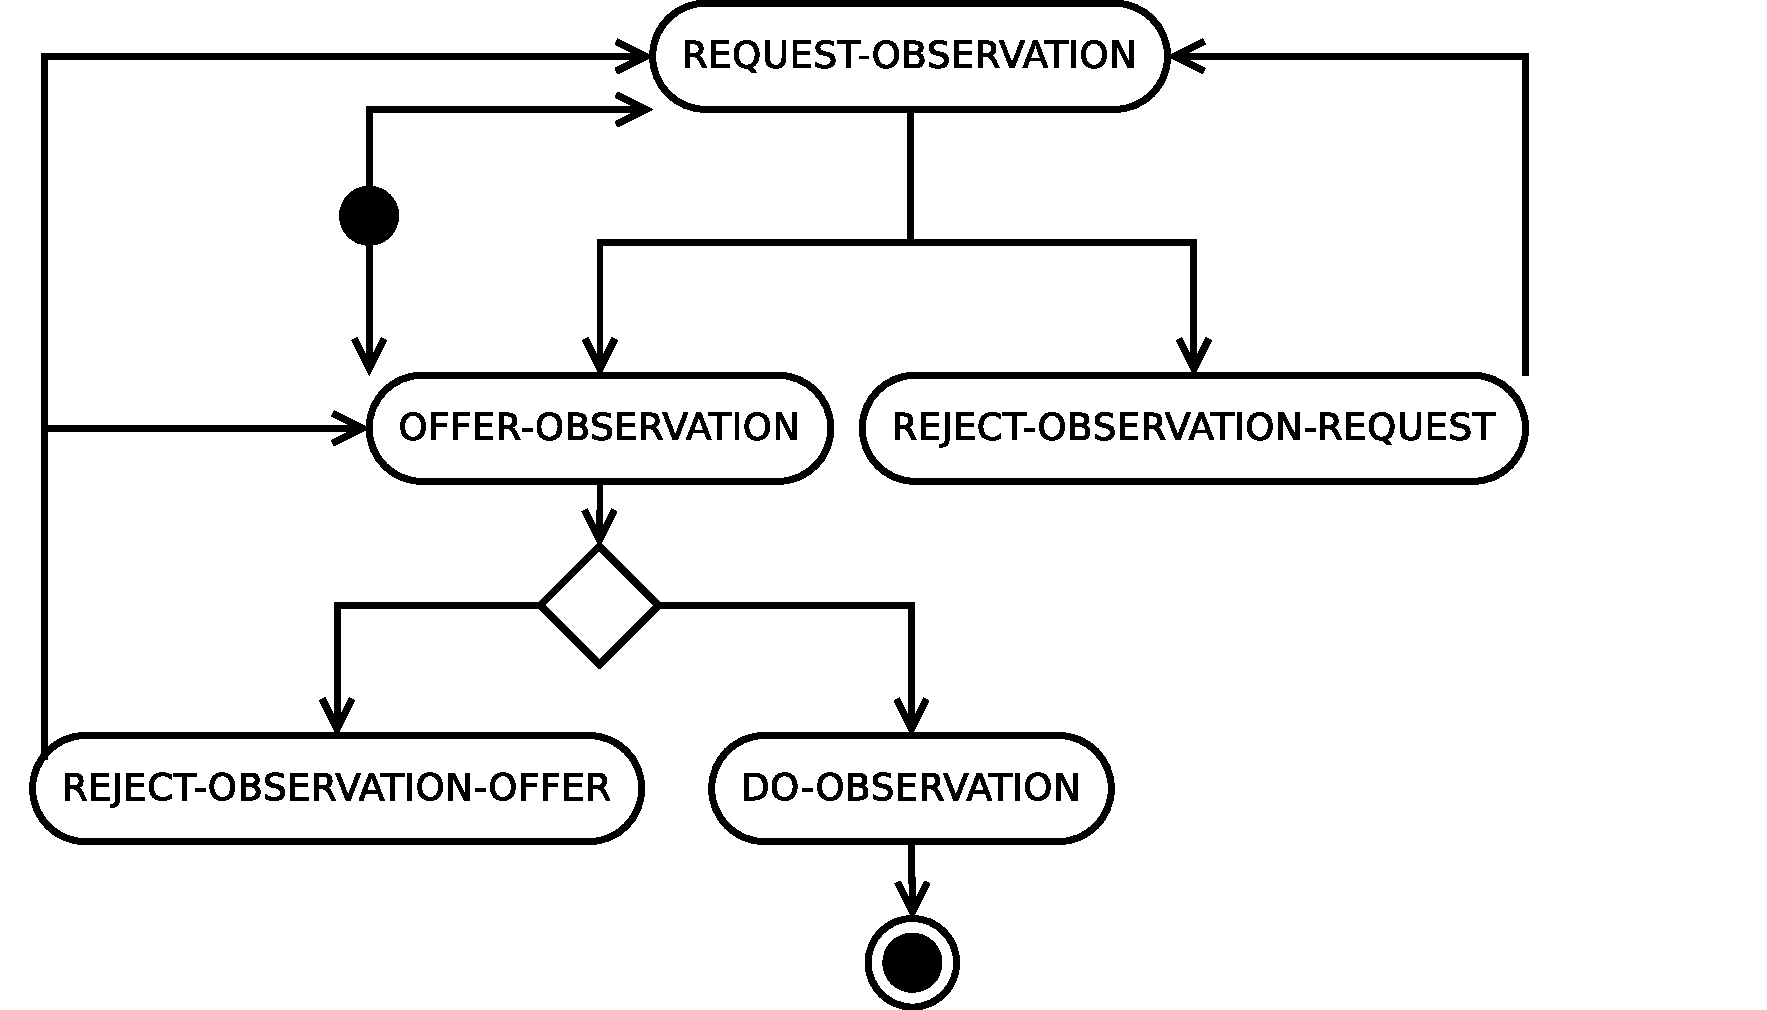
\includegraphics[width=1.00\textwidth]{trans3-control.pdf}
	\caption{Control flow of the negotiate observable transaction}
	\label{fig:trans3-control}
\end{figure}




\noindent
\begin{tabular}{|>{\colleft}p{3cm}|>{\colleft}p{8.5cm}|} \hline
{\bf Communication model} 	& {\bf Information Exchange Specification Worksheet CM-2} \\ \hline \hline
\sc Transaction 			& \emph{Transaction 4: Report observable} \\ \hline
\sc Agents involved 		& 1. {\bf Sender}(Car repair assistant): Observation result options  \newline
					  2. {\bf Receiver}(Hobbyist): Observation result options \newline
					  3. {\bf Sender}(Hobbyist): Observation result \newline
					  4. {\bf Receiver}(Car repair assistant): Observation result \\ \hline
					  
\multicolumn{2}{|l|}{\textsc{Information items}} \\ \hline
   					%List all information items that are to be transmitted in this
   					%transaction. This includes the (`core') information object the
   					%transfer of which is the purpose of the transaction. However, it may contain
   					%other, supporting, information items, that, for example, provide help
   					%or explanation. For each information item, describe the following:
OBSERVATION RESULT OPTIONS	&  1. {\bf Role}: A support information object. \newline
					% whether it is a {\em core} object, or a {\em support} item.
					   2. {\bf Form}: List of strings  \newline
					% the syntactic form in which it transmitted to another agent , e.g., data string, canned text, a certain type of diagram, 2D or 3D plot.
					   3. {\bf Medium}: Varies, it might be a menu or it might be a free form with suggestions noted separately\\ 
					% the medium through which it is handled in the agent-agent interaction, e.g., a pop-up window, navigation and selection within a menu, command-line interface, human intervention.
OBSERVATION RESULT		&  1. {\bf Role}: A core information object. \newline
					   2. {\bf Form}: Varies, it might be a identifier, a number or a string. \newline
					   3. {\bf Medium}: Varies, it might be selection in a menu or it might be typed in a field.\\ \hline
					
\multicolumn{2}{|l|}{\textsc{Message specifications}}\\ \hline
					% Describe all messages that make up the transaction. For each individual message describe:
OPTION-MESSAGE			& {\bf Communication type}: ASK \newline
					% the communication type of the message describing its intention (``illocutionary force,'' in speech-act terminology). 
					  {\bf Content}: Observation result options and the request to provide the actual observation result \newline
					% the statement or proposition contained in the message.
					% {\bf Reference}: car repair information\newline
					%in certain cases, it may be useful to add a reference to, for example, what domain knowledge model or agent capability is required to be able to send or process the message.
					  {\bf From}: Car repair assistant\newline
					  {\bf To}: Hobbyist\\ \hline
					  
OBSERVATION-MESSAGE		& {\bf Communication type}: REPLY \newline
					% the communication type of the message describing its intention (``illocutionary force,'' in speech-act terminology). 
					  {\bf Content}: The observation result \newline
					% the statement or proposition contained in the message.
					% {\bf Reference}: car repair information\newline
					%in certain cases, it may be useful to add a reference to, for example, what domain knowledge model or agent capability is required to be able to send or process the message.
					  {\bf From}: Hobbyist\newline
					  {\bf To}: Car repair assistant\\ \hline
%\sc Control over messages 	& \\ \hline
   					%Give, if necessary, a control specification over the messages
   					%within the transaction. This can be done in pseudocode format or
   					%in a state-transition diagram, similar to how the control over
   					%transaction within the communication plan is specified. The
   					%difference is just the level of detail.
\end{tabular}



\noindent
\begin{tabular}{|>{\colleft}p{3cm}|>{\colleft}p{8.5cm}|} \hline
{\bf Communication model} 	& {\bf Information Exchange Specification Worksheet CM-2} \\ \hline \hline
\sc Transaction 			& \emph{Transaction 5: Report hypothesis} \\ \hline
\sc Agents involved 		& 1. {\bf Sender}(Car repair assistant): Hypothesis  \newline
					  2. {\bf Sender}(Car repair assistant): Hypothesis argumentation \newline
					  3. {\bf Sender}(Car repair assistant): Repair plan \newline
					  4. {\bf Receiver}(Hobbyist): Hypothesis \newline
					  5. {\bf Receiver}(Hobbyist): Hypothesis argumentation \newline
					  6. {\bf Receiver}(Hobbyist): Repair plan \\ \hline
					  
\multicolumn{2}{|l|}{\textsc{Information items}} \\ \hline
   					%List all information items that are to be transmitted in this
   					%transaction. This includes the (`core') information object the
   					%transfer of which is the purpose of the transaction. However, it may contain
   					%other, supporting, information items, that, for example, provide help
   					%or explanation. For each information item, describe the following:
HYPOTHESIS				&  1. {\bf Role}: A core information object. \newline
					% whether it is a {\em core} object, or a {\em support} item.
					   2. {\bf Form}: A string stating the hypothesis \newline
					% the syntactic form in which it transmitted to another agent , e.g., data string, canned text, a certain type of diagram, 2D or 3D plot.
					   3. {\bf Medium}: Displayed in the main window\\ 
					% the medium through which it is handled in the agent-agent interaction, e.g., a pop-up window, navigation and selection within a menu, command-line interface, human intervention.
HYPOTHESIS ARGUMENTATION	&  1. {\bf Role}: A support information object. \newline
					   2. {\bf Form}: A list of strings each stating one reasoning step \newline
					   3. {\bf Medium}: Displayed in the main window\\
REPAIR PLAN				&  1. {\bf Role}: A support information object. \newline
					   2. {\bf Form}: A text, possibly with images\newline
					   3. {\bf Medium}: Displayed in the main window\\ \hline
					
\multicolumn{2}{|l|}{\textsc{Message specifications}}\\ \hline
					% Describe all messages that make up the transaction. For each individual message describe:
HYPOTHESIS-MESSAGE		& {\bf Communication type}: REPORT \newline
					% the communication type of the message describing its intention (``illocutionary force,'' in speech-act terminology). 
					  {\bf Content}: The hypothesis, the hypotheses argumentation and the repair plan (plan depending on car repair information)\newline
					% the statement or proposition contained in the message.
					  {\bf Reference}: car repair information\newline
					%in certain cases, it may be useful to add a reference to, for example, what domain knowledge model or agent capability is required to be able to send or process the message.
					  {\bf From}: Hobbyist\newline
					  {\bf To}: Car repair assistant\\ \hline
					  
%\sc Control over messages 	& \\ \hline
   					%Give, if necessary, a control specification over the messages
   					%within the transaction. This can be done in pseudocode format or
   					%in a state-transition diagram, similar to how the control over
   					%transaction within the communication plan is specified. The
   					%difference is just the level of detail.
\end{tabular}